\documentclass{article}

\usepackage{fancyhdr}
\usepackage{extramarks}
\usepackage{amsmath}
\usepackage{amsthm}
\usepackage{amsfonts}
\usepackage{tikz}
\usepackage[plain]{algorithm}
\usepackage{algpseudocode}
\usepackage{placeins}

\usetikzlibrary{automata,positioning}

%
% Basic Document Settings
%

\topmargin=-0.45in
\evensidemargin=0in
\oddsidemargin=0in
\textwidth=6.5in
\textheight=9.0in
\headsep=0.25in

\linespread{1.1}

\pagestyle{fancy}
\lhead{\hmwkAuthorName}
\chead{\hmwkClass\: \hmwkTitle}
\rhead{\firstxmark}
\lfoot{\lastxmark}
\cfoot{\thepage}

\renewcommand\headrulewidth{0.4pt}
\renewcommand\footrulewidth{0.4pt}

\setlength\parindent{0pt}

\newtheorem{subproblem}{Subproblem}

%
% Create Problem Sections
%

\newcommand{\enterProblemHeader}[1]{
    \nobreak\extramarks{}{Problem \arabic{#1} continued on next page\ldots}\nobreak{}
    \nobreak\extramarks{Problem \arabic{#1} (continued)}{Problem \arabic{#1} continued on next page\ldots}\nobreak{}
}

\newcommand{\exitProblemHeader}[1]{
    \nobreak\extramarks{Problem \arabic{#1} (continued)}{Problem \arabic{#1} continued on next page\ldots}\nobreak{}
    \stepcounter{#1}
    \nobreak\extramarks{Problem \arabic{#1}}{}\nobreak{}
}

\setcounter{secnumdepth}{0}
\newcounter{partCounter}
\newcounter{homeworkProblemCounter}
\setcounter{homeworkProblemCounter}{1}
\nobreak\extramarks{Problem \arabic{homeworkProblemCounter}}{}\nobreak{}

%
% Homework Problem Environment
%
% This environment takes an optional argument. When given, it will adjust the
% problem counter. This is useful for when the problems given for your
% assignment aren't sequential. See the last 3 problems of this template for an
% example.
%
\newenvironment{homeworkProblem}[1][-1]{
    \ifnum#1>0
        \setcounter{homeworkProblemCounter}{#1}
    \fi
    \section{Problem \arabic{homeworkProblemCounter}}
    \setcounter{partCounter}{1}
    \enterProblemHeader{homeworkProblemCounter}
}{
    \exitProblemHeader{homeworkProblemCounter}
}

%
% Homework Details
%   - Title
%   - Due date
%   - Class
%   - Section/Time
%   - Instructor
%   - Author
%

\newcommand{\hmwkTitle}{Past Paper May 2013}
\newcommand{\hmwkDueDate}{April 24, 2023}
\newcommand{\hmwkClass}{ASR}
\newcommand{\hmwkAuthorName}{\textbf{Patrick Tourniaire}}

%
% Title Page
%

\title{
    \vspace{2in}
    \textmd{\textbf{\hmwkClass:\ \hmwkTitle}}\\
    \normalsize\vspace{0.1in}\small{Completed\ on\ \hmwkDueDate}\\
    \vspace{3in}
}

\author{\hmwkAuthorName}
\date{}

\renewcommand{\part}[1]{\textbf{\large Part \Alph{partCounter}}\stepcounter{partCounter}\\}

%
% Various Helper Commands
%

% Useful for algorithms
\newcommand{\alg}[1]{\textsc{\bfseries \footnotesize #1}}

% For derivatives
\newcommand{\deriv}[1]{\frac{\mathrm{d}}{\mathrm{d}x} (#1)}

% For partial derivatives
\newcommand{\pderiv}[2]{\frac{\partial}{\partial #1} (#2)}

% Integral dx
\newcommand{\dx}{\mathrm{d}x}

% Alias for the Solution section header
\newcommand{\solution}{\textbf{\large Solution}}

% Probability commands: Expectation, Variance, Covariance, Bias
\newcommand{\E}{\mathrm{E}}
\newcommand{\Var}{\mathrm{Var}}
\newcommand{\Cov}{\mathrm{Cov}}
\newcommand{\Bias}{\mathrm{Bias}}

\begin{document}

\maketitle

\pagebreak


% Problem 1
\begin{homeworkProblem}
    
    % Sub-problem 1
    \begin{subproblem} 
        Why is a pre-emphasis filter of the following form applied to the speech signal?
        \begin{align} \label{math_env:/pre-emphasis-modified}
            x[n'] = x[n] + \alpha x[n-1]
        \end{align}
    \end{subproblem}
    
    \textbf{Answer}

    Pre-emphasis is a processing method which increases the amplitude of high frequency bands
    and decreases the amplitudes of lower bands. The traditional formulation for pre-emphasis
    is given by Equation \ref{math_env:/pre-emphasis}.

    \begin{align} \label{math_env:/pre-emphasis}
        x[n'] = x[n] - \alpha x[n-1]
    \end{align}

    Which measure the transition between signal timesteps, whereas Equation 
    \ref{math_env:/pre-emphasis-modified} further exagerates this by not subtracting the previous
    amplitude. Therefore, the pre-emphasis of this given form is a first order high-pass filter
    which amplifies the high frequency components of the signal. It achieves this by adding a scaled
    version of the previous sample to the current sample.


    % Sub-problem 2
    \begin{subproblem}
        Why is a Hamming window often used rather than a rectangular window? In your answer sketch the shape of each window in the time domain and sketch the effect of each on a sine wave of constant frequency.
    \end{subproblem}

    \textbf{Answer}

    A Hamming window is often used rather than a rectangular window in signal processing because it 
    helps reduce the effects of spectral leakage and improve the frequency resolution.

    \begin{figure}[h]
        \minipage{0.48\textwidth}
            \centering
            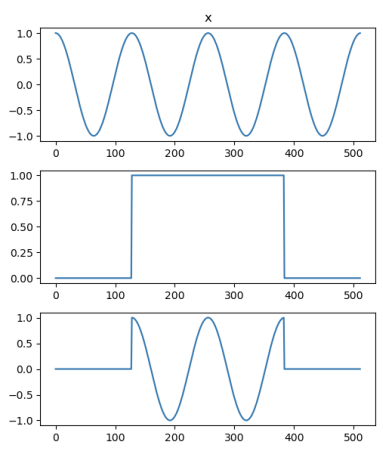
\includegraphics[width=\textwidth]{figures/rect-window.png}
            \caption{Rectangular window effect}
            \label{fig:/rect-window}
        \endminipage\hfill
        \minipage{0.48\textwidth}
            \centering
            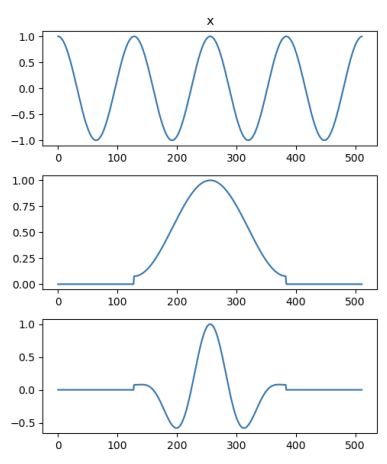
\includegraphics[width=\textwidth]{figures/hamming-window.png}
            \caption{Hamming window effect}
            \label{fig:/hamming-window}
        \endminipage\hfill
    \end{figure}

    As we can observe in Figure \ref{fig:/rect-window}, the rectangular window will potentially 
    introduce a large drop in the signal amplitude which is intrepreted as spectral leakage. However,
    for the Hammming window we do not observe this pattern as highlighted by Figure \ref{fig:/hamming-window}.
    Since this window filter has a slight taper at the ends as opposed to the drastic drop for the rectangular
    window, we get a smoother filtering of the sinus wave.    


    % Sub-problem 3
    \begin{subproblem}
        How does a mel-scale filter bank model the human perception of frequency?
    \end{subproblem}

    \textbf{Answer}

    The mel-scale filter bank model is a model of human audotory perception that aims to simulate the
    way we hear and process sound by being more discriminative at lower bands and more discriminatory
    at higher bands. Which mimicks the non-liniarity of the human audotory system. In Figure 
    \ref{fig:/mel-scale-model} we can observe how this model prioritises lower frequencies.

    \begin{figure}[h]
        \centering
        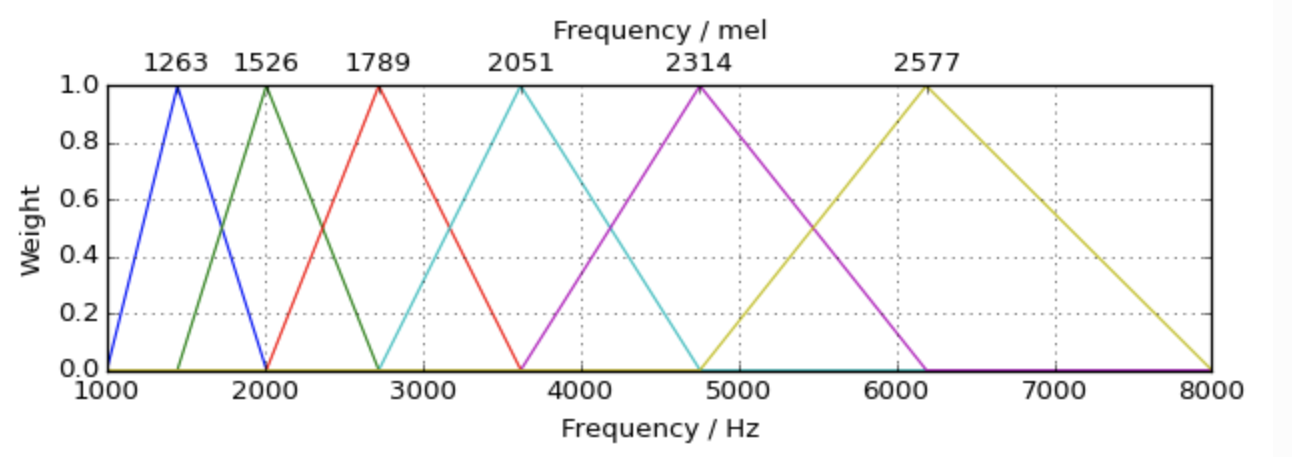
\includegraphics[width=0.80\textwidth]{figures/mel-scale-model.png}
        \caption{Mel-scale filter bank model example}
        \label{fig:/mel-scale-model}
    \end{figure}
    
    Additionally, we observe that the length of the triangles in the lower frequencies are smaller,
    which will result in more frequencies being canceled and reduced significantly. Whereas the higher
    frequencies have longer triangles, thus ensuring that a larger range of frequencies are accounted for.
    Which highlighs how model indeed follows the non-liniarity of the human auditory system.

    
    % Sub-problem 4
    \begin{subproblem}
        What is cepstral analysis and how is it used to seperate source and filter characteristics in speech?
    \end{subproblem}

    \textbf{Answer}

    Cepstral analysis is used as the power spectrum of a signal has some useful properties for seperating
    the source and filter in a signal. We define the source and filter by the following.
    
    \begin{itemize}
        \item \textbf{Source:} refers to the vocal cords and the way they vibrate to produce sound.
        \item \textbf{Filter:} shape and characteristic of the vocal tract that modify the sound produced by the vocal cords.
    \end{itemize}

    Cepstral analysis is therefore used to seperate the characteristics of source and filter by decomposing
    the log spectrum of the speech signal into its constituent parts. The cepstrum process looks like the following.

    \begin{enumerate}
        \item Compute the FFT (fast-fourier transform) of the speech signal to obtain its frequency spectrum.
        \item Compute the power spectrum of the speech signal by taking the magnitude squared of the FFT.
        \item Take the log of the power spectrum to obtain the log spectrum.
        \item Take the inverse fourier transform of the log spectrum to obtain the cepstrum.
        \item Analyse the cepstrum to separate the source and filter characteristics of the speech signal.
    \end{enumerate}

    The first few coefficients correspond to the filter characteristics of the speech signal, while the later 
    coefficients correspond to the source characteristics. The plot over the different coefficients can be observed
    in Figure

    \begin{figure}[!t]
        \centering
        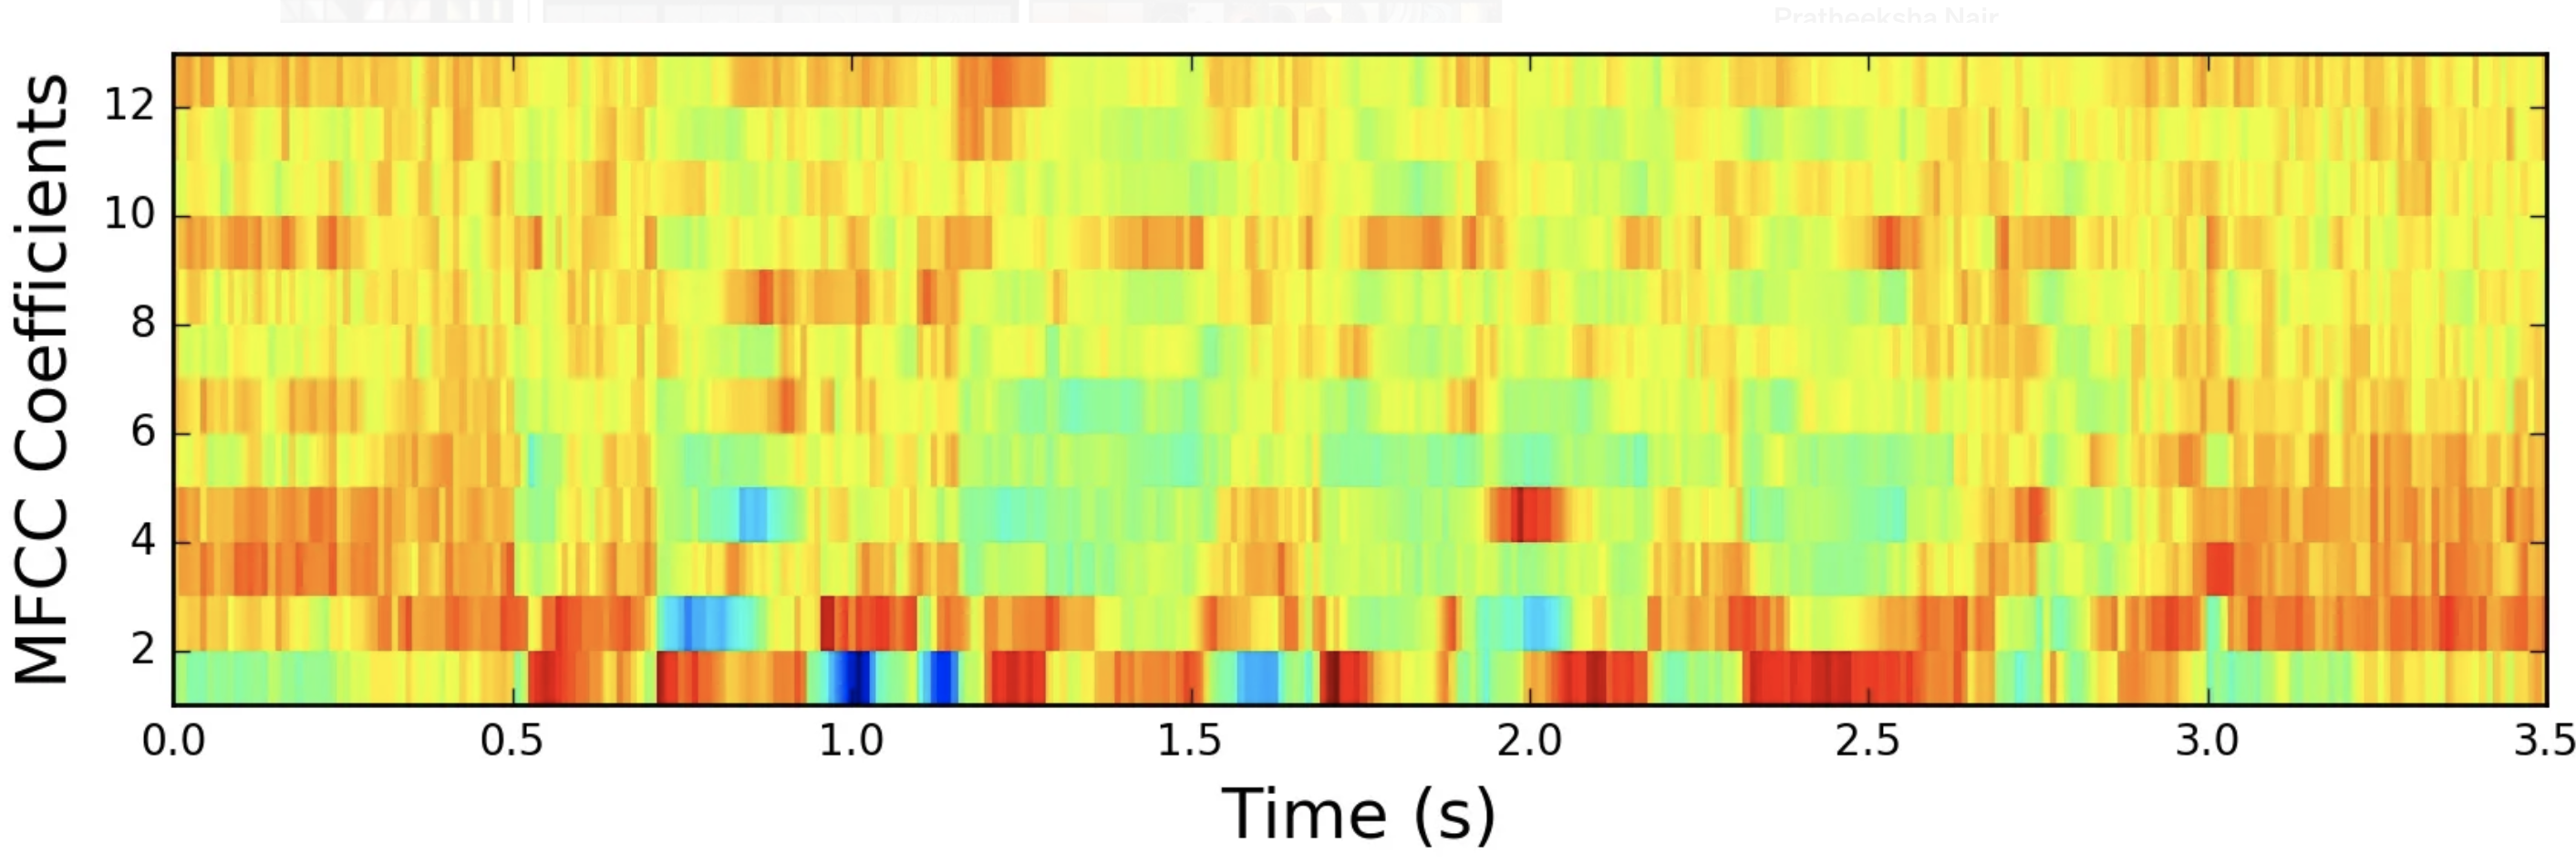
\includegraphics[width=0.80\textwidth]{figures/cepstrum.png}
        \caption{MFCC plot with the cepstrum coefficients}
        \label{fig:/mfcc-plot}
    \end{figure}
    \FloatBarrier
    

    % Sub-problem 5
    \begin{subproblem}
        Consider an HMM with an output distribution given by a (single) Gaussian per state. We would like to estimate 
        the Gaussian mean vector $\mu_j$ of state $s_j$, given a training sequence of acoustic observations 
        $X = x_1, \ldots, x_t, \ldots, x_T$. In Viterbi training the time-state alignment is assumed to be known. Write 
        an expression for the maximum likelihood estimate of $\mu_j$.
    \end{subproblem}

    \textbf{Answer}
    
    The expression for the estimated $\mu_j$, given that we have a single Gaussian optimised using MLE is given by.

    \begin{align}
        \hat{\mu}_j = \dfrac{1}{T} \displaystyle\sum_{i=0}^{T} x_i
    \end{align}

    
    % Sub-problem 6
    \begin{subproblem}
        In the case where the time-state alignment is not known, the EM algorithm may be used to estimate the mean vector. 
        The EM algorithm makes use of the state occupation probability of state $s_j$ at time $t$, $\gamma_t(s_j)$, where $s_j$
        is a state of the HMM.

        \begin{itemize}
            \item Express $\gamma_t(s_j)$ as a conditional probability.
            \item How may $\gamma_t(s_j)$ be written in terms of the forward and backward probabilities?
            \item Explain how $\gamma_t(s_j)$ may be used to re-estimate $\mu_j$.
        \end{itemize}
    \end{subproblem}

    \textbf{Answer}

    We can express $\gamma_t(s_j)$ as a conditional probability by the following expression.

    \begin{align}
        \gamma_t(s_j) &= P(q_t = j | X, M) \intertext{Recalling that $P(X | M) = \alpha_E$ we can express this term
        by the forward ($\alpha$) and backward probabilities ($\beta$), where $M$ represents the HMM topology.}
        &= \dfrac{1}{\alpha_E} \alpha_j(s_j) \beta_j(s_j)
    \end{align}

    For re-estimating the means of the state Gaussians, we can can treat the occupation probabilities as priors representing the
    likelihood of some RV realisation $x$ belonging to some Gaussian component $j$. Thus, the estimation for parameter $\mu$ becomes.

    \begin{align}
        \hat{\mu}_{j} = \displaystyle\frac{\sum_{t=0}^{T} \gamma_t(s_j) x_t}{\sum_{t=0}^{T} \gamma_t(s_j)}
    \end{align}

    
    % Sub-problem 7
    \begin{subproblem}
        Why are HMM computations usually performed in the log domain?
    \end{subproblem}

    \textbf{Answer}

    HMM computations are performed in the log domain due to the fact that we have to deal with long likelihood chains
    which are multiplied together to estimate the parameters of the model. However, the problem with this is that this can
    result in incredibly small numbers which inturn can result in float compuation errors when the computer performs the
    computation. Therefore, we convert to logs as then the multiplication essentially becomes the same as an addition of log
    likelihoods, as the following property applies.

    \begin{align}
        log(a b) = log(a) + log(b)
    \end{align}
\end{homeworkProblem}


% Problem 2
\begin{homeworkProblem}

    % Sub-problem 1
    \begin{subproblem}
        Describe two ways that neural networks trained to perform phone recognition can be used to provide discriminative features for HMM/GMM speech recognition systems (tandem systems).
    \end{subproblem}

    \textbf{Answer}

    One way neural networks trained for phone recognition can be used to provide discriminative features for HMM/GMM 
    speech recognition systems is through a tandem approach. In this approach, the neural network is used as a
    front-end feature extracttor for the HMM/GMM system. The output of the neural network, which is typically a set of
    bottleneck features, is concatenated with the traditional MFCC features exctracted from the speech signal. The
    concatenated features are then used as input to the HMM/GMM system for phone recognition.

    Another way neural network can be used to provide discriminative features for HMM/GMM speech recognition systems is
    through a hybrid approach. In this approach, a neural network is used to estimate the posterior probability of the
    phone labels given the acoustic features. These posteriors are then used as input to the HMM/GMM system as a replacement
    for the traditional Gaussian micture model likelihood scores. The HMM/GMM system can then use these posteriors to
    estimate the most likely phone sequence given the input speech signal. This approach has been shown to improve phone
    recognition performance, particularly in noisy environments.


    % Sub-problem 2
    \begin{subproblem}
        Consider a hybrid HMM / neural network system.
        \begin{itemize}
            \item How do hybrid systems differ from tandem systems?
            \item In a context-independent hybrid HMM / neural network system, why
            is the neural network output corresponding to phone $q$, divided by an
            estimate of the prior probability $P(q)$?
        \end{itemize}
    \end{subproblem}

    A tandem system of a neural network and a HMM/GMM, results in a system where the neural network supplies additional
    features for the HMM/GMM system to use. Which is done by concatenating the features to the traditional MFCC features.
    On the other hand, a hybrid approach will simply use the features of the neural network, where it outputs posterior
    probabilities for the phones given the features.

    In a context-independent hybrid HMM/NN system, the neural network is used to estimate the posterior probability of a
    phone given the acoustic features. The posterior probability of a phone is the probability of the phone given the
    observed features, and it is proportional to the product of the likelihood of the features given the phone and the
    prior probability of the phone.

    In this context-independent system, the prior probability of each phone is assumed to be equal. However, in reality,
    some phones occur more frequently than others in the training data. Therefore, dividing the NN output corresponding to
    phone $q$ by an estimate of the prior probability $P(q)$ helps to normalise the ouput and make it less biased towards
    the more frequent phones. This is known as Bayesian normalisation, and it ensures that the output of the NN is proportional
    to the likelihood of the features given the phone, and not influenced by the prior probability of the phone.

    By normalizing the output in this way, the hybrid system can effectively estimate the posterior probability of a phone given
    the observed features, which can be used to improve phone recognition accuracy.


    % Sub-problem 3
    \begin{subproblem}
        Consider a context-dependent hybrid HMM / neural network system.
        \begin{itemize}
            \item For practical purposes, a context-dependent HMM/GMM system is required before beginning to train a hybrid system. Why is this so?
            \item Compare and contrast two methods of performing speaker adaptation in a context-dependent hybrid system.
        \end{itemize}
    \end{subproblem}

    \textbf{Answer}

    A context-dependent HMM/GMM system is required before training a hybrid system because it provides the necessary context-dependent
    labels that the NN needs to learn the mapping between the acoustic features and the corresponding phone labels. 
    Conext-independent HMM/GMM systems assume that each phone has a fixed acoustic representation that is independent
    of its context. However, in reality, the acoustic realisation of a phone depends on the context in which it appears. For example,
    the acoustic realisation of the phone /t/ may be different in the word "then" compared to the word "stop". Therefore,
    context-dependent HMM/GMM systems use different models for each phone depending on the surrounding context, which captures the
    contextual variations of each phone.

    The outputs of a context dependent HMM/GMM system are context-dependent phone labels, which are used to train the NN in the hybrid
    system. The NN learns to map the context-dependent acoustic features to the corresponding context-dependent phone labels, which
    improves the accuracy of phone recognition. Therefore, a context-dependent HMM/GMM system is required before training a hybrid system
    to provide the context-dependent phone labels that the NN needs to learn the mapping between the acoustic features and the corresponding
    phone labels.

    As people have varied pronounciations and different accents, single pre-trained models can struggle to pick up such variances. Therefore, we
    introduce a technique called speaker adaption. Which for a context-dependent model such as the HMM/GMM can have two approaches for achieving
    speaker adaption, namely feature-space transforms and model-based adaption. Feature-space transforms involve transforming the input acoustic 
    features of a speaker into a space that is better aligned with the average acoustic characteristics of the training data. One common 
    feature-space transform method is maximum likelihood linear regression (MLLR), which learns a linear transformation matrix to adapt 
    the acoustic model for a specific speaker. MLLR has been shown to be effective for speaker adaptation in context-dependent hybrid systems, 
    especially when a small amount of speaker-specific training data is available.

    Model-based adaptation involves adapting the parameters of the acoustic model directly using speaker-specific training data. One common 
    model-based adaptation method is speaker-adaptive training (SAT), which involves retraining the acoustic model using speaker-specific data. 
    SAT has been shown to be effective for speaker adaptation in context-dependent hybrid systems, especially when a large amount of 
    speaker-specific training data is available. A major difference between feature-space transforms and model-based adaptation is the amount 
    of speaker-specific data required. \textit{Feature-space transforms can be effective even with a small amount of speaker-specific training data}, 
    while \textit{model-based adaptation requires a larger amount of speaker-specific data to be effective}. \textit{However, model-based adaptation can 
    potentially achieve higher accuracy than feature-space transforms, especially when a large amount of speaker-specific training data is 
    available.}

    In summary, both feature-space transforms and model-based adaptation are effective methods for speaker adaptation in context-dependent hybrid 
    systems, but they differ in the amount of speaker-specific data required and the potential accuracy gains. Feature-space transforms can be effective
    with a small amount of speaker-specific data, while model-based adaptation requires more data but can potentially achieve higher accuracy.


    % Sub-problem 4
    \begin{subproblem}
        It might be possible to obtain better acoustic likelihood estimates by combining HMM/GMM and hybrid HMM / neural network systems. How could this be done at the frame level?
    \end{subproblem}

    \textbf{Answer}
    
    Yes, this is possible and one way to achieve this would be to have a HMM/GMM model which estimates the likelihood of the acoustic observation
    given the hidden state. Then, the neural network can further refine these estimates based on the features extracted from the acoustic signals.
    One way would be to use a feed-forward neural network which takes the HMM/GMM output as input, and then generates a refined likelihood estimate
    based on the output.

    Another approach is to use a recurrent neural network (RNN) as the neural component of the hybrid system. The RNN would take as input a sequence 
    of frames and their corresponding HMM/GMM likelihood estimates, and generate a sequence of refined likelihood estimates. This approach is 
    particularly useful when modeling long-term dependencies in the acoustic signal.
    
\end{homeworkProblem}


% Problem - 3
\begin{homeworkProblem}

    % Sub-problem 1
    \begin{subproblem}
        What is multistyle training and how does it improve noise-robustness? What are its drawbacks?
    \end{subproblem}

    \textbf{Answer}

    Multistyle training is a technique which is used to make the model more adaptable to noise, by training it on multiple speaking styles and many 
    different acoustic environments. Whereas a traditional approach would imply that the model is trained on a single speaking environment and a
    single way of pronounciating. In short, this style of tranining improves noise-robustness by doing the following three things, exposes the model
    to a wider range of acoustic environments which enambles it to work even in noisy environments. A larger collection of different pronounciations
    which will enable it to work for non-native people, thirdly it can help reduce overfitting as there are many different speaking styles and environments
    which enables the model to generalise better.

    However, there are some drawbacks to such a model and training style. Since it requires a multiple environments and speaking styles then this means
    that the for each style we need many datapoints. Thus making the model computationally expensive and time-consuming. This can lead to the model
    performing worse for certain speaking styles and environments, particularly if the dataset is not balanced. Further, multi-task training might not
    work for all kinds of noise data, therefore we might require additional training styles or techniques for addressing noise in data.


    % Sub-problem 2
    \begin{subproblem}
        What is spectral subtraction and how does it address noise-robustness? What are its drawbacks?
    \end{subproblem}

    \textbf{Answer}

    Spectral subtraction is used often for noise-reduction. This is done by removing the noise component of a speech signal by subtracting away the
    estimate of the noise spectrum from the observed speech spectrum. This resulting cleaned speech spectrum can then be used for performing automatic
    speech recognition. The noise-estimated spectrum is usually obtained by training a model to produce such estimates by using a noise only dataset.
    The noise-estimated spectrum is then subtracted away from the observed speech spectrum on a frequency basis. The resulting speectrum is then passed
    through an inverse Fourier transform.

    Spectral subtraction can improve noise-robustness in several ways. First, it can remove noise from the speech signal, which can improve the accuracy 
    of subsequent speech processing tasks such as speech recognition or speaker identification. Second, it can improve the quality of the speech signal, 
    making it more intelligible and easier to understand. Third, it is a relatively simple and computationally efficient technique, making it easy to 
    implement in real-time speech processing systems. However, spectral subtraction has some drawbacks. One major drawback is that it assumes that the 
    noise spectrum is stationary, which may not be true in practice. If the noise is non-stationary or varies over time, spectral subtraction may not 
    be able to effectively remove the noise component from the speech signal. Additionally, spectral subtraction can introduce distortion or artifacts 
    in the cleaned speech signal, particularly if the noise spectrum estimate is inaccurate or if the subtraction process is not properly calibrated. 
    Finally, spectral subtraction can sometimes result in a loss of speech information or intelligibility, particularly if the noise is very strong or 
    if the speech signal is very low in volume.


    % Sub-problem 3
    \begin{subproblem}
        How does discriminative training of the acoustic model of an HMM/GMM
        speech recognition system differ from maximum likelihood parameter
        estimation? Why does discriminative training usually increase speech
        recognition accuracy?
    \end{subproblem}

    \textbf{Answer}

    Discriminative training of the acoustic model in an HMM/GMM speech recognition system differs from maximum likelihood parameter estimation in 
    that it aims to directly optimize the model's ability to discriminate between different speech classes or targets, rather than simply maximizing 
    the likelihood of the training data. Maximum likelihood parameter estimation involves estimating the parameters of the HMM/GMM model by maximizing 
    the likelihood of the training data, given the model. This approach does not explicitly take into account the discriminative power of the model, 
    and can result in a model that is not well-suited to the particular task of speech recognition.

    Discriminative training, on the other hand, directly optimizes the model's ability to discriminate between different speech classes or targets, 
    such as different phonemes or words. This is typically done by minimizing an objective function that measures the difference between the model's 
    predicted output and the true target output. This approach can lead to a model that is better tailored to the specific task of speech recognition, 
    and can improve the model's ability to distinguish between similar-sounding speech sounds. Discriminative training usually increases speech 
    recognition accuracy because it explicitly optimizes the model's ability to discriminate between different speech sounds, and can therefore lead 
    to a model that is better able to handle the variability in speech sounds caused by factors such as speaking style, accent, and background noise. 
    Additionally, discriminative training can improve the robustness of the model to variations in the training data, and can lead to better 
    generalization performance on unseen data.


    % Sub-problem 4
    \begin{subproblem}
        Write down the objective function that is optimised in maximum mutual
        information estimation (MMIE), and explain its relation to the objective
        function used in maximum likelihood estimation (MLE).
    \end{subproblem}

    \textbf{Answer}

    Maximum mutual information estimation (MMIE) is an approach to training the parameters of a speech recognition system that aims to directly 
    optimize the mutual information between the speech input and the corresponding output labels. The MMIE approach is similar to maximum likelihood 
    estimation (MLE) in that it seeks to estimate the model parameters that maximize the likelihood of the training data. However, MMIE introduces a 
    regularization term that encourages the model to learn to produce more accurate posterior probabilities for the output labels, leading to better 
    discrimination between different classes. The objective function used in MMIE is given by:

    \begin{align}
        F_{MMIE} &= \displaystyle\sum_{u=1}^{U} log P_{\lambda} (M(W_u) | \textbf{X}_u) \\
                 &= \displaystyle\sum_{u=1}^{U} log \displaystyle\frac{P_{\lambda} (\textbf{X}_u | M(W_u)) P (W_u)}{\sum_{w'} P_{\lambda} (\textbf{X}_u | M(w'_u)) P(w'_u)}
    \end{align}


    % Sub-problem 5
    \begin{subproblem}
        How does minimum phone error (MPE) training differ from MMIE?
    \end{subproblem}

    \textbf{Answer}

    
\end{homeworkProblem}

\end{document}
